\documentclass[12pt,a4paper]{article}
\usepackage[utf8]{inputenc}
\usepackage[spanish,es-tabla]{babel}
\usepackage{geometry}
\usepackage{graphicx}
\usepackage{multirow}
\usepackage{tabularx}
\usepackage{mathptmx}
\usepackage{fancyhdr}
\usepackage{array}
\usepackage[table]{xcolor}
\usepackage{titlesec}
\usepackage{setspace}
\usepackage{microtype}
\usepackage{lastpage}
\usepackage{booktabs}
\usepackage{enumitem}
\usepackage{amsmath}
\usepackage{amsfonts}
\usepackage{amssymb}

\graphicspath{{images/}{../images/}{./}}

\geometry{
    top=4.7cm,
    bottom=2.5cm,
    left=2.5cm,
    right=2.5cm,
    headheight=3.9cm,
    headsep=0.4cm
}

\setstretch{1.15}
\setlength{\parindent}{0pt}
\setlength{\parskip}{0.45em}
\setlength{\tabcolsep}{4pt}

\titleformat{\section}
  {\normalfont\fontsize{12}{14.5}\bfseries}{\thesection.}{0.6em}{\uppercase}
\titlespacing*{\section}
  {0pt}{1.8ex plus 0.4ex minus 0.2ex}{0.6ex plus 0.2ex}

\titleformat{\subsection}
  {\normalfont\fontsize{11.5}{13.5}\bfseries}{\thesubsection.}{0.5em}{}
\titlespacing*{\subsection}
  {0pt}{1.4ex plus 0.3ex minus 0.1ex}{0.4ex plus 0.1ex}

\titleformat{\subsubsection}
  {\normalfont\fontsize{10.5}{12.5}\bfseries\itshape}{\thesubsubsection.}{0.4em}{}
\titlespacing*{\subsubsection}
  {0pt}{1.1ex plus 0.2ex minus 0.1ex}{0.3ex plus 0.1ex}

\newcolumntype{Y}{>{\centering\arraybackslash}X}
\newcolumntype{L}{>{\raggedright\arraybackslash}X}
\newcolumntype{C}{>{\centering\arraybackslash}X}

\definecolor{headerblue}{RGB}{26, 54, 93}
\definecolor{darkblue}{RGB}{43, 108, 176}
\definecolor{lightgraybg}{RGB}{248, 248, 248}
\definecolor{tableheader}{RGB}{232, 238, 246}

\newcommand{\docCodigo}{TI-SIGE-ENT-F2-002}
\newcommand{\docVersion}{1.0}
\newcommand{\docProceso}{ARQUITECTURA DE SOFTWARE / SAD Y C4}
\newcommand{\docElaboracion}{28/08/2026}
\newcommand{\docRevision}{28/08/2026}
\newcommand{\docTitulo}{DISEÑO DE ARQUITECTURA DE LA SOLUCIÓN}
\newcommand{\docOrganizacion}{FACULTAD DE INGENIERÍA EN SISTEMAS, ELECTRÓNICA E INDUSTRIAL}
\newcommand{\docSubOrganizacion}{CARRERA DE INGENIERÍA DE SOFTWARE}

\newcommand{\encabezadofrecuente}{%
    \renewcommand{\arraystretch}{1.15}%
    \noindent\makebox[\textwidth][c]{%
    \begin{tabularx}{\textwidth}{|>{\centering\arraybackslash}m{2.8cm}|Y|>{\centering\arraybackslash}m{4.8cm}|}
        \hline
        \multirow{4}{2.8cm}{\centering\raisebox{-1.15cm}{
\includegraphics[width=2.5cm,height=2.0cm,keepaspectratio]{images/logo.png}}}
        & \textbf{\fontsize{9}{11}\selectfont \docOrganizacion} 
        & \textbf{\fontsize{8}{10}\selectfont CÓDIGO:} \fontsize{8}{10}\selectfont \docCodigo \\
        \cline{3-3}
        & \textbf{\fontsize{8.5}{10.5}\selectfont \docSubOrganizacion} 
        & \textbf{\fontsize{8}{10}\selectfont VERSIÓN:} \fontsize{8}{10}\selectfont \docVersion \\
        \cline{2-3}
        & \textbf{\fontsize{8}{10}\selectfont PROCESO:} \fontsize{8}{10}\selectfont \docProceso 
        & \textbf{\fontsize{8}{10}\selectfont ELABORACIÓN:} \fontsize{8}{10}\selectfont \docElaboracion \\
        \cline{2-3}
        & \textbf{\fontsize{8.5}{10.5}\selectfont \docTitulo} 
        & \textbf{\fontsize{8}{10}\selectfont ÚLTIMA REVISIÓN:} \fontsize{8}{10}\selectfont \docRevision \\
        \hline
    \end{tabularx}%
    }%
}

\pagestyle{fancy}
\fancyhf{}
\fancyhead[C]{\encabezadofrecuente}
\fancyfoot[C]{\fontsize{10}{12}\selectfont Página \thepage\ de \pageref{LastPage}}
\renewcommand{\headrulewidth}{0pt}

\begin{document}

\noindent{\fontsize{10.5}{12.5}\selectfont \textbf{Integrantes:} Heidi Villavicencio \quad$\vert$\quad Steeven Toala \quad$\vert$\quad Nixon Hurtado \quad$\vert$\quad Andrea Vásquez}

\vspace{0.25cm}

\section{Título}
\textbf{Denominación del Entregable:} Documento de Arquitectura de Software (SAD \& C4 Model) -- Código EDT: 2.2

\section{Introducción}
La arquitectura de software constituye el esquema estructural y de organización técnica que determina la robustez, escalabilidad y mantenibilidad de la solución SIGE. En este documento se formaliza el \\textbf{Software Architecture Document (SAD)} fundamentado en los principios de Clean Architecture (Arquitectura Limpia) y el modelo C4 (Contexto, Contenedores, Componentes y Código). Se detalla la separación estricta de responsabilidades entre el Dominio institucional, los Casos de Uso de Aplicación, los Adaptadores de Infraestructura (PostgreSQL 18, MinIO S3, LanguageTool) y la capa de Presentación Web RESTful.

\section{Objetivo}
\subsection{Objetivo General}
Diseñar la arquitectura técnica de la solución SIGE basada en principios de desacoplamiento, inmutabilidad y alta cohesión, documentada mediante el modelo C4 y vistas arquitectónicas estándar.
\subsection{Objetivos Específicos}
\begin{itemize}[leftmargin=1.5em, itemsep=2pt]
    \item Estructurar las 4 capas de la Arquitectura Limpia: Dominio, Aplicación, Infraestructura y API.
    \item Elaborar los diagramas C4 de Nivel 1 (Contexto de Sistema) y Nivel 2 (Contenedores).
    \item Definir los patrones de diseño: Repository Pattern, Mediator, Middleware Pipeline y CQRS.
\end{itemize}

\section{Alcance}
\subsection{Límites del Entregable (In-Scope)}
\begin{itemize}[leftmargin=1.5em, itemsep=2pt]
    \item Diseño de arquitectura de microservicios contenerizados y tuberías de middlewares en Express v5.
    \item Estrategia de persistencia en PostgreSQL 18 y almacenamiento desacoplado de objetos en MinIO S3.
\end{itemize}
\subsection{Exclusiones (Out-of-Scope)}
\begin{itemize}[leftmargin=1.5em, itemsep=2pt]
    \item Arquitecturas de microservicios distribuidos en múltiples clústeres Kubernetes (excede el alcance del VPS local).
\end{itemize}

\section{Definiciones}
\begin{itemize}[leftmargin=1.5em, itemsep=2pt]
    \item \textbf{Clean Architecture:} Paradigma arquitectónico donde las reglas de negocio de la entidad no dependen de ningún framework externo.
    \item \textbf{C4 Model:} Jerarquía visual para la arquitectura de software (Contexto, Contenedores, Componentes y Código).
    \item \textbf{Repository Pattern:} Patrón que desacopla la lógica de negocio del acceso y persistencia en la base de datos.
    \item \textbf{Middleware Pipeline:} Cadena secuencial de interceptores de solicitudes HTTP para validación, autenticación y registro.
\end{itemize}

\section{Responsabilidades}
\begin{itemize}[leftmargin=1.5em, itemsep=2pt]
    \item \textbf{Steeven Toala (Responsable EDT 2.2):} Definición de capas arquitectónicas, diagramación C4 y selección de patrones de diseño.
    \item \textbf{Nixon Hurtado (Backend):} Revisión de adaptadores de infraestructura y base de datos.
    \item \textbf{Ing. Paulo Torres (Docente Evaluador):} Aprobación del SAD institucional.
\end{itemize}

\section{Normativa Legal y Técnica}
\begin{itemize}[leftmargin=1.5em, itemsep=2pt]
    \item \textbf{ISO/IEC/IEEE 42010:2011:} Systems and software engineering -- Architecture description.
    \item \textbf{The Open Group Architecture Framework (TOGAF 9.2).}
\end{itemize}

\section{Método, Políticas y Contenidos}
Se aplicó modelado C4. En las Figuras \ref{fig:s2_02_clean} y \ref{fig:s2_02_c4} se presentan el diagrama de capas de Arquitectura Limpia y el diagrama C4 de Contenedores.

\begin{figure}[htbp]
    \centering
    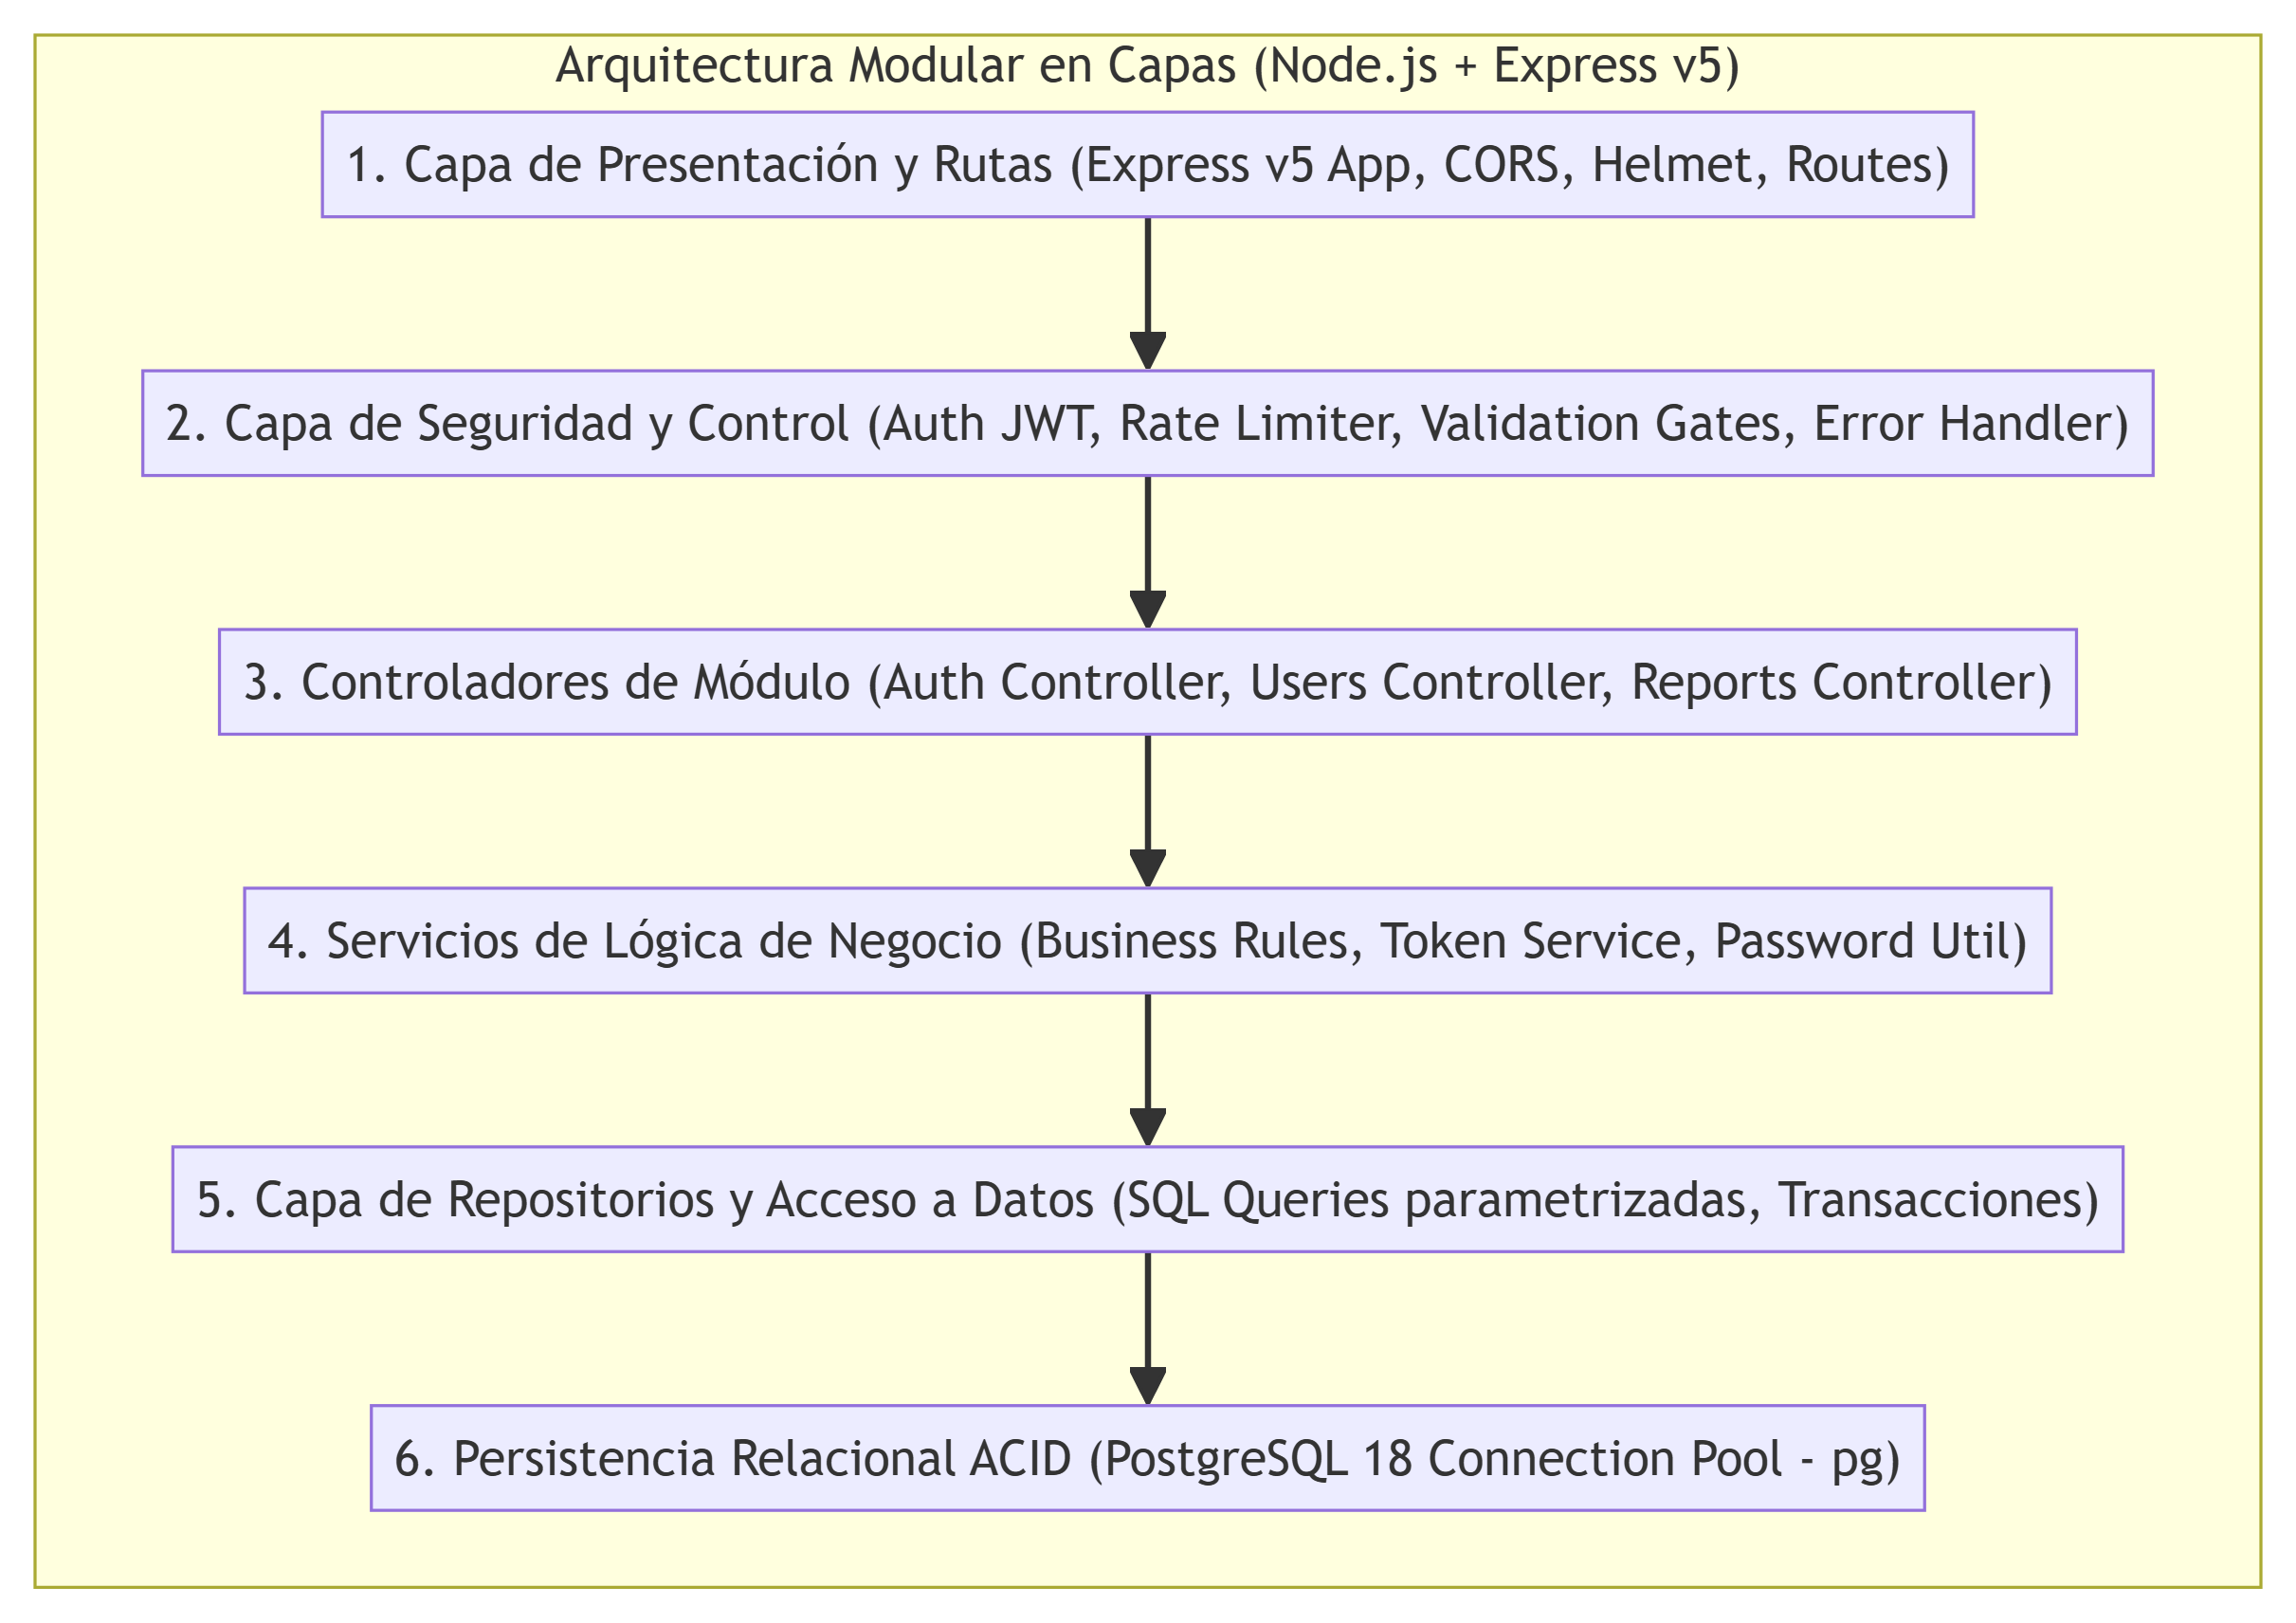
\includegraphics[width=0.85\textwidth,height=5.2cm,keepaspectratio]{images/s2_02_clean_architecture.png}
    \caption{Arquitectura Limpia del Sistema SIGE (Capas y Regla de Dependencia).}
    \label{fig:s2_02_clean}
\end{figure}

\begin{figure}[htbp]
    \centering
    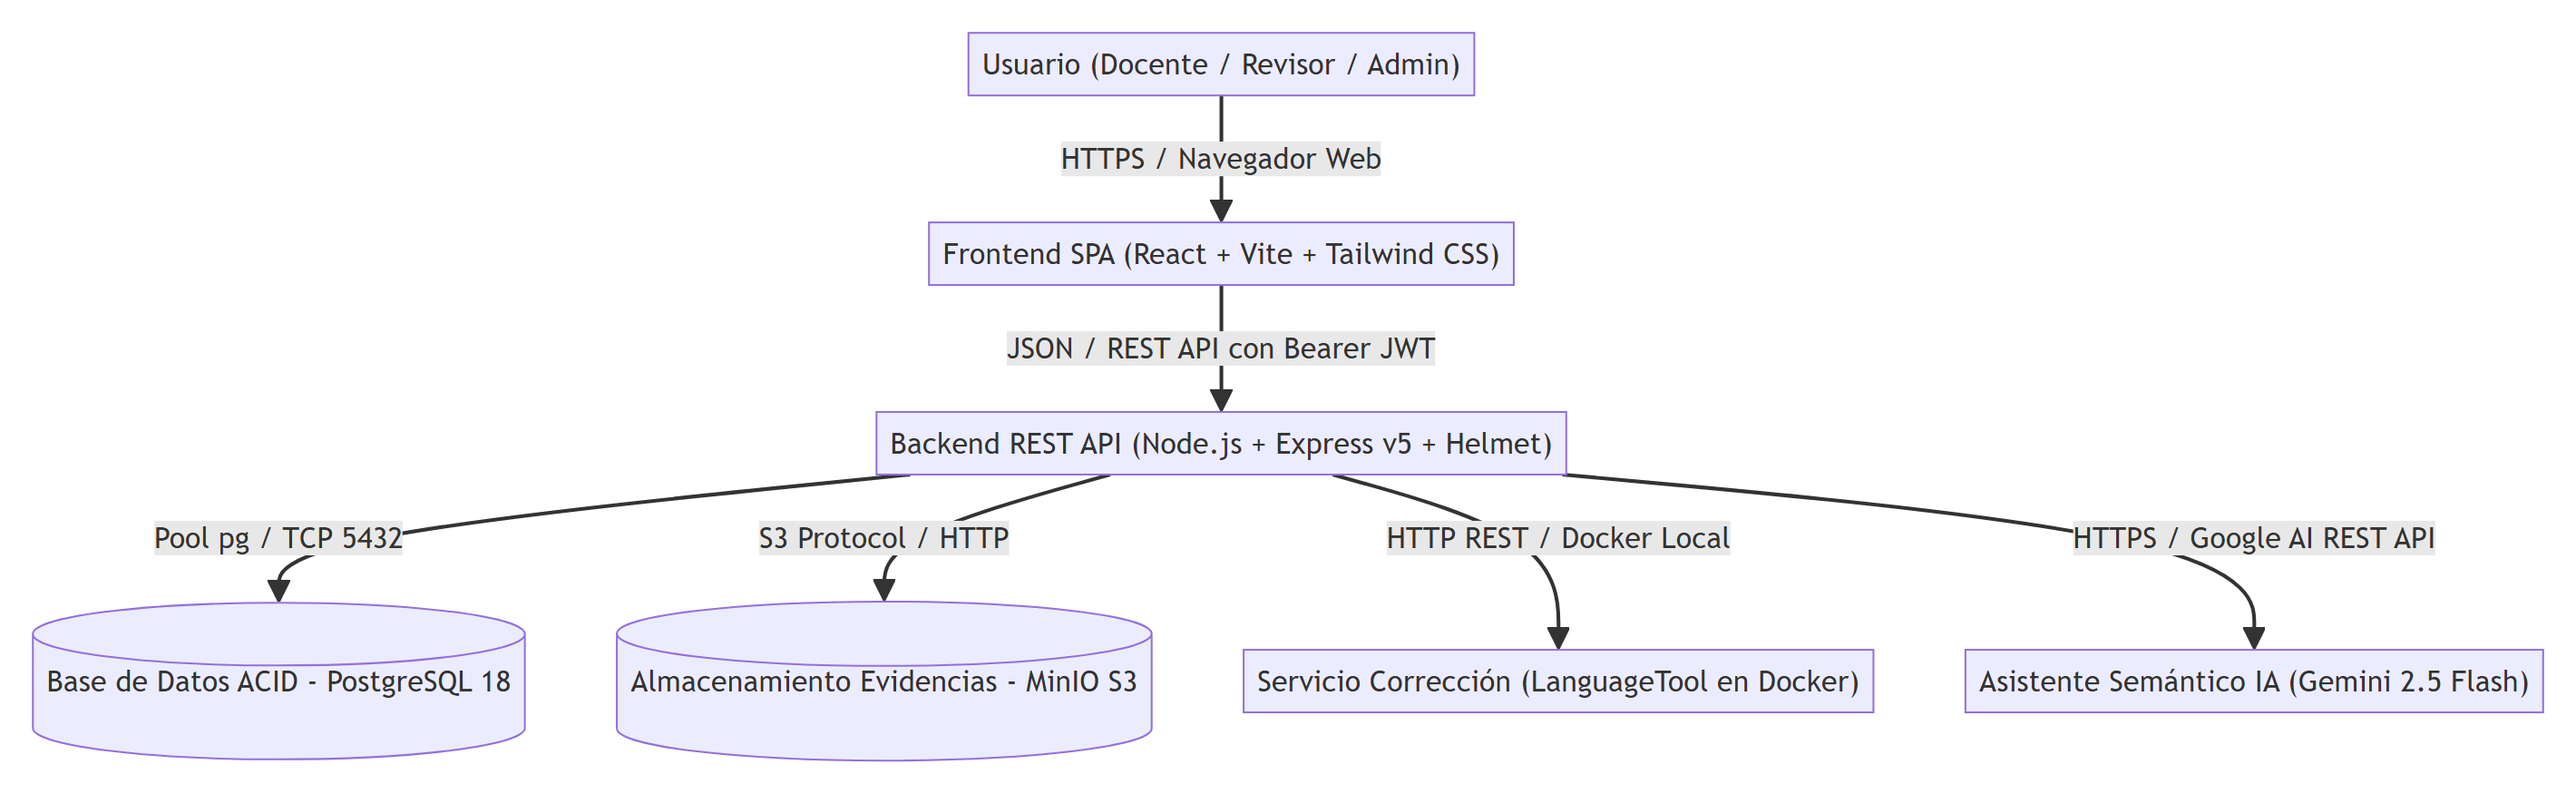
\includegraphics[width=0.88\textwidth,height=5.5cm,keepaspectratio]{images/s2_02_contenedores_c4.png}
    \caption{Diagrama C4 de Nivel 2: Contenedores y Protocolos de Comunicación.}
    \label{fig:s2_02_c4}
\end{figure}

\section{Descripción de actividades}
\subsection{Organización de Capas de la Arquitectura Limpia}
\begin{table}[htbp]
\centering
\small
\renewcommand{\arraystretch}{1.2}
\begin{tabularx}{\textwidth}{|>{\bfseries}m{3.2cm}|X|X|}
\hline
\rowcolor{tableheader}
\textbf{Capa Arquitectónica} & \textbf{Responsabilidad Primaria} & \textbf{Componentes Clave} \\
\hline
1. Domain (Núcleo) & Entidades puras de negocio y reglas inmutables del SGC. Cero dependencias de librerías externas. & Entidad Documento, Actividad, Validación Ponderación ($100\%$), Firma Digital. \\
\hline
2. Application & Orquestación de casos de uso, transacciones y lógica de flujo documental. & Servicios de Documentos, Flujo de Firmas, Motor de Validation Gates. \\
\hline
3. Infrastructure & Adaptadores tecnológicos externos, bases de datos y servicios de red. & Repositorio PostgreSQL 18, MinIO Storage Client, LanguageTool REST Client, Google Gemini API Client. \\
\hline
4. Presentation / API & Interfaz gráfica SPA y endpoints HTTP RESTful con middlewares de seguridad. & Express v5 REST API, Auth JWT Middleware, SPA React + Vite + Tailwind CSS. \\
\hline
\end{tabularx}
\caption{Capas y Responsabilidades de la Arquitectura del Sistema SIGE.}
\label{tab:capas_arch}
\end{table}

\subsection{Estrategia de Seguridad e Inmutabilidad}
Toda mutación de estado que legalice un documento genera un sellado digital con el cálculo del hash criptográfico del contenido consolidado, imposibilitando la alteración retroactiva de datos en base de datos.

\section{Firmas de Responsabilidad}

\noindent
\renewcommand{\arraystretch}{1.2}
\begin{tabularx}{\textwidth}{|>{\raggedright\arraybackslash}m{2.9cm}|>{\raggedright\arraybackslash}X|>{\centering\arraybackslash}m{4.6cm}|>{\centering\arraybackslash}m{2.3cm}|}
    \hline
    \rowcolor{tableheader}
    \textbf{ACCIÓN} & \textbf{NOMBRE Y CARGO} & \textbf{FIRMA} & \textbf{FECHA} \\
    \hline
    \textbf{Elaborado por:} & Heidi Villavicencio\newline Analista de Calidad / UI-UX & \parbox[c]{4.4cm}{\centering\vspace{4pt}
\includegraphics[height=1.5cm,width=4.0cm,keepaspectratio]{images/firma_heidi.png}\vspace{4pt}} & 28/08/2026 \\
    \hline
    \textbf{Revisado por:} & Steeven Toala\newline Líder de Proyecto / Arquitecto & \parbox[c]{4.4cm}{\centering\vspace{4pt}
\includegraphics[height=1.5cm,width=4.0cm,keepaspectratio]{images/firma_steveen.png}\vspace{4pt}} & 28/08/2026 \\
    \hline
    \textbf{Aprobado por:} & Ing. Paulo Torres, Mg.\newline Docente Evaluador -- Gestión Proyectos & \parbox[c]{4.4cm}{\centering\vspace{8pt}\textbf{\textcolor{gray!80}{\scriptsize [ PENDIENTE DE APROBACIÓN ]}}\vspace{8pt}} & \textbf{\textcolor{gray!90}{Pendiente}} \\
    \hline
\end{tabularx}

\vspace{0.4cm}

\section{Control de Cambios}

\noindent
\renewcommand{\arraystretch}{1.2}
\begin{tabularx}{\textwidth}{|>{\hsize=0.45\hsize\centering\arraybackslash}X|>{\hsize=1.55\hsize\raggedright\arraybackslash}X|>{\hsize=1.2\hsize\raggedright\arraybackslash}X|>{\hsize=0.8\hsize\centering\arraybackslash}X|}
    \hline
    \rowcolor{tableheader}
    \textbf{Versión} & \textbf{Descripción del cambio} & \textbf{Responsable del cambio} & \textbf{Fecha de aprobación} \\
    \hline
    1.0 & Emisión inicial del entregable según EDT del Tablero Trello & Equipo de Proyecto SIGE & 28/08/2026 \\
    \hline
\end{tabularx}

\vspace{0.4cm}

\section{Anexos}
\begin{itemize}[leftmargin=1.5em]
\item \textbf{Anexo 1:} Ficha Técnica de Decisión Arquitectónica (ADR-01 a ADR-05).
\end{itemize}

\end{document}
